\documentclass[border=10pt]{standalone}
\usepackage{tikz,amsmath}
\usetikzlibrary{arrows.meta}
\usepackage{tikzcats}   % 原生保留 tikzcats

% ========== 画布级字号 ==========
\newcommand{\bigf}{\fontsize{26}{32}\selectfont}
\newcommand{\smallf}{\fontsize{22}{28}\selectfont}
\newcommand{\tinyf}{\fontsize{20}{26}\selectfont}

% ========== 配色 ==========
\definecolor{hidFill}{RGB}{199,203,243}
\definecolor{hidLine}{RGB}{52,58,143}
\definecolor{inFill}{RGB}{183,224,177}
\definecolor{inLine}{RGB}{32,102,32}
\definecolor{orFill}{RGB}{250,224,180}
\definecolor{orLine}{RGB}{190,110,20}
\definecolor{outFill}{RGB}{243,199,199}
\definecolor{outLine}{RGB}{143,52,52}
\colorlet{hid}{hidLine}
\colorlet{in}{inLine}
\colorlet{or}{orLine}
\colorlet{out}{outLine}

\begin{document}
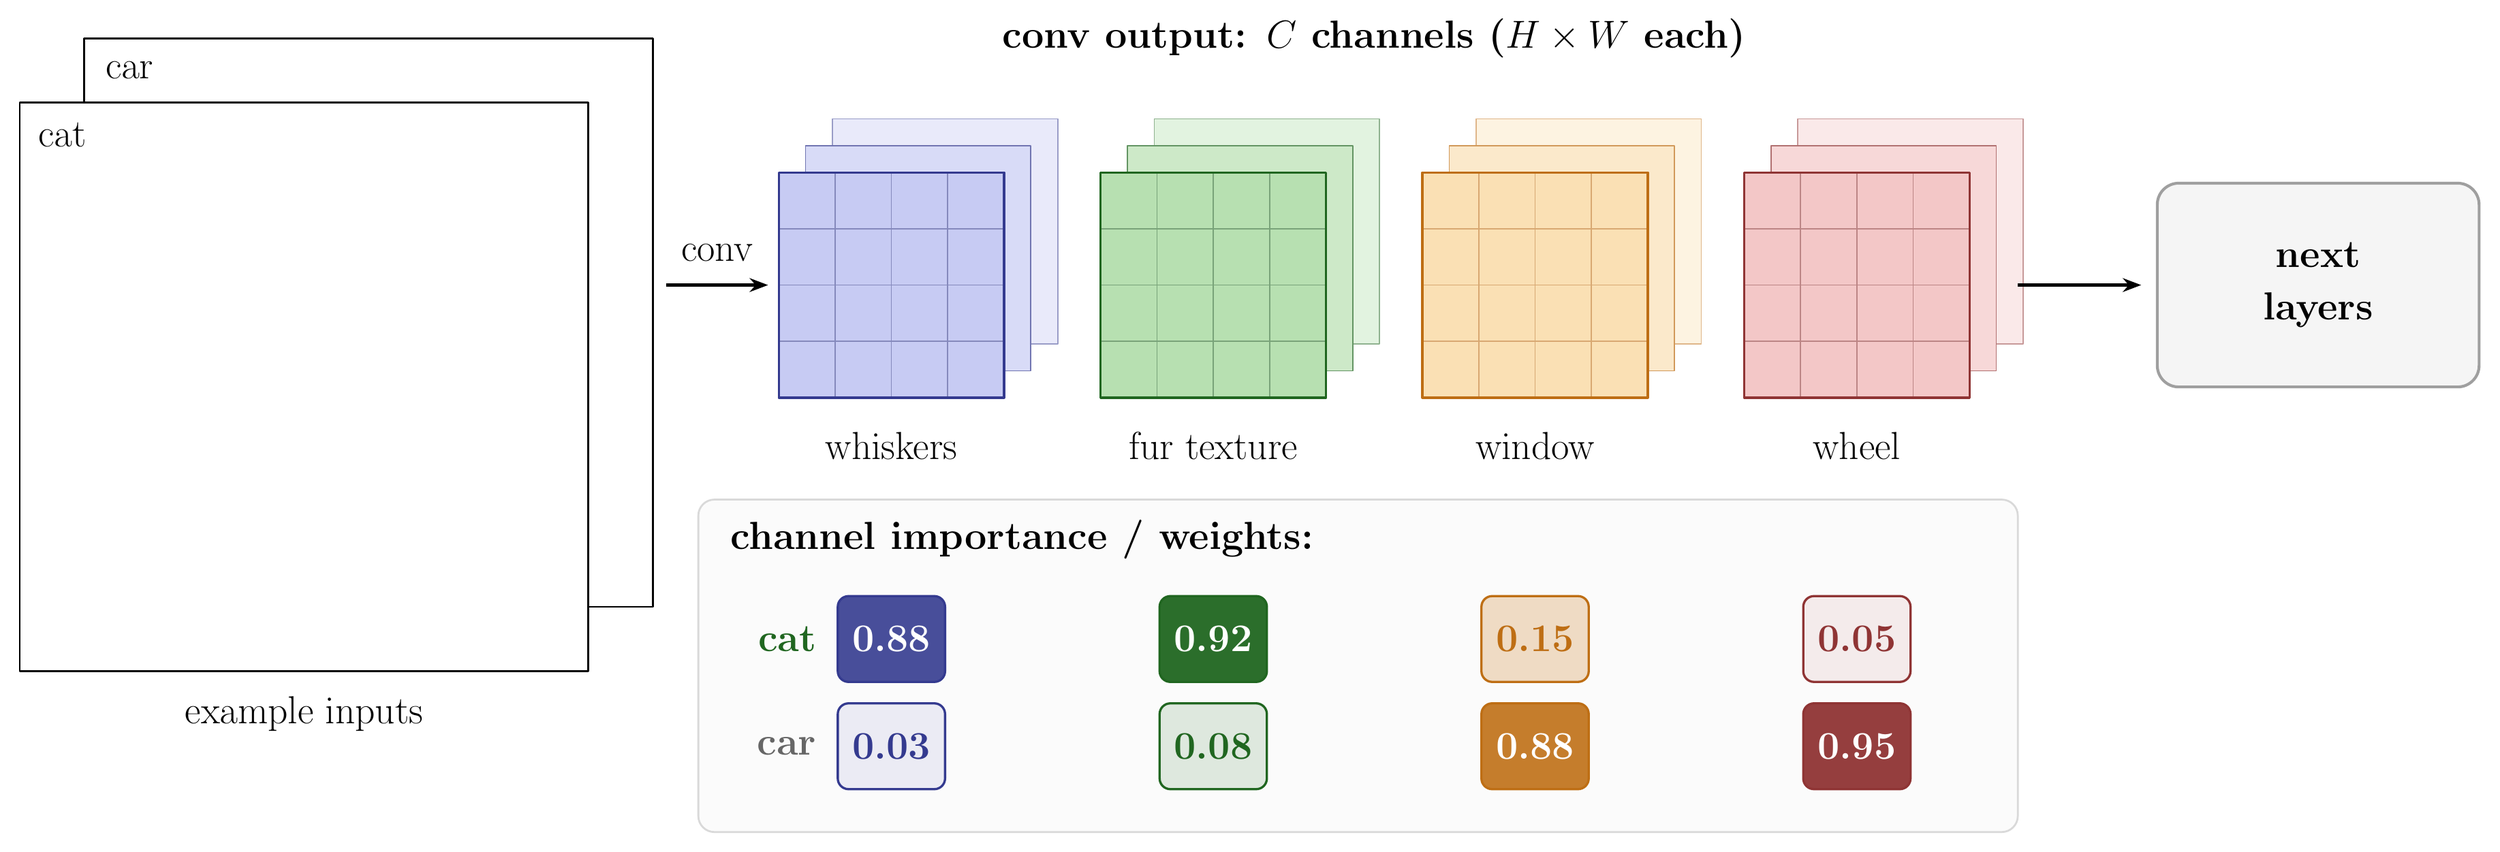
\begin{tikzpicture}[
    font=\bigf, line join=round,
    every node/.style={inner sep=0pt, outer sep=0pt, align=center},
    arr/.style={->, >=Stealth, line width=1.5pt}
  ]

  % ========== 宏 ==========
  \newcommand{\gridbox}[5]{%
    \fill[#5Fill] (#1,#2) rectangle ++(#3*#4, #3*#4);
    \draw[step=#4, #5Line!60, line width=.6pt, shift={(#1,#2)}] (0,0) grid (#3*#4, #3*#4);
    \draw[#5Line, line width=1.2pt] (#1,#2) rectangle ++(#3*#4, #3*#4);
  }
  
  \newcommand{\stack}[3]{%
    \fill[#3Fill!40, draw=#3Line!50, line width=.6pt] ({#1+1.0},{#2+1.0}) rectangle ++(4*1.05, 4*1.05);
    \fill[#3Fill!70, draw=#3Line!70, line width=.6pt] ({#1+0.5},{#2+0.5}) rectangle ++(4*1.05, 4*1.05);
    \gridbox{#1}{#2}{4}{1.05}{#3}
  }

  % ========== 输入：两张堆叠照片 (原样保留) ==========
  \draw[black, line width=1pt, fill=white] (0.55,9.0) rectangle (11.15,19.6);
  \node[font=\tinyf, anchor=west] at (0.95,19.0) {car};
  \draw[black, line width=1pt, fill=white] (-0.65,7.8) rectangle (9.95,18.4);
  \begin{scope}[shift={(5.8,15.4)}] \cat \end{scope}
  \node[font=\tinyf, anchor=west] at (-0.3,17.8) {cat};
  \node[font=\smallf] at (4.65,7.0) {example inputs};

  % ========== 卷积箭头 ==========
  \draw[arr] (11.4,15) -- (13.3,15);
  \node[font=\smallf] at (12.35,15.6) {conv};

  % ========== 四个通道：堆叠网格 ==========
  \node[font=\smallf\bfseries] at (24.6,19.6) {conv output: $C$ channels ($H\times W$ each)};
  \stack{13.5}{12.9}{hid}
  \stack{19.5}{12.9}{in}
  \stack{25.5}{12.9}{or}
  \stack{31.5}{12.9}{out}
  
  % 通道特征名称
  \node[font=\smallf] at (15.6,12.0) {whiskers};
  \node[font=\smallf] at (21.6,12.0) {fur texture};
  \node[font=\smallf] at (27.6,12.0) {window};
  \node[font=\smallf] at (33.6,12.0) {wheel};

  % ========== 通道重要性 (框上移一半，且内部标题与内容行距拉开) ==========
  \draw[draw=gray!30, fill=gray!3, rounded corners=3mm, line width=1pt] (12.0, 4.8) rectangle (36.6, 11.0);
  \node[font=\smallf\bfseries, anchor=west] at (12.6, 10.25) {channel importance / weights:};

  % cat 权重条 (上边距拉开，块位于 7.6 ~ 9.2)
  \node[font=\smallf\bfseries, text=inLine, anchor=east] at (14.2, 8.4) {cat};
  \foreach \x/\col/\op/\val/\tc in {15.6/hid/90/0.88/white, 21.6/in/95/0.92/white, 27.6/or/25/0.15/orLine, 33.6/out/10/0.05/outLine} {
    \fill[\col!\op, draw=\col, line width=1.2pt, rounded corners=2mm] (\x-1.0, 7.6) rectangle ++(2.0, 1.6);
    \node[font=\smallf\bfseries, text=\tc] at (\x, 8.4) {\val};
  }

  % car 权重条 (块位于 5.6 ~ 7.2)
  \node[font=\smallf\bfseries, text=gray!80!black, anchor=east] at (14.2, 6.4) {car};
  \foreach \x/\col/\op/\val/\tc in {15.6/hid/10/0.03/hidLine, 21.6/in/15/0.08/inLine, 27.6/or/90/0.88/white, 33.6/out/95/0.95/white} {
    \fill[\col!\op, draw=\col, line width=1.2pt, rounded corners=2mm] (\x-1.0, 5.6) rectangle ++(2.0, 1.6);
    \node[font=\smallf\bfseries, text=\tc] at (\x, 6.4) {\val};
  }

  % ========== 右侧：下一层 ==========
  \draw[arr] (36.6,15) -- (38.9,15);
  \node[draw=gray!75, fill=gray!8, line width=1.5pt, rounded corners=4mm, minimum width=6cm, minimum height=3.8cm, font=\smallf\bfseries]
    at (42.2,15) {next\\layers};

\end{tikzpicture}
\end{document}